\documentclass[10pt, a4paper]{article}
\usepackage{lrec}
%\usepackage{multibib}
%\newcites{languageresource}{Language Resources}
\usepackage{graphicx}
\usepackage{tabularx}
\usepackage{soul}
% for eps graphics
\usepackage[usenames, dvipsnames]{color}

\usepackage{epstopdf}
\usepackage[latin1]{inputenc}
\usepackage{xspace}
\usepackage{booktabs}
\usepackage{hyperref}
\usepackage{xstring}
\usepackage{xspace}
\usepackage{multirow}
\usepackage{colortbl}


\newcommand{\secref}[1]{\StrSubstitute{\getrefnumber{#1}}{.}{ }}

\newcommand{\refexp}[1]{\textsl{#1}}
\newcommand{\word}[1]{\textsl{#1}}
\newcommand{\cat}[1]{\textsc{#1}}
\newcommand{\vgenome}{VisualGenome\xspace}
\newcommand{\vg}{VG\xspace}
\newcommand{\ra}{$\rightarrow$}
\newcommand{\referit}{ReferIt\xspace}
\newcommand{\refcoco}{RefCOCO\xspace}
\newcommand{\refcocop}{RefCOCO+\xspace}
\newcommand{\flickr}{Flickr30k Entities\xspace}

\newcommand{\sz}[1]{\textcolor{blue}{\emph{//sz: #1//}}}
\newcommand{\gbt}[1]{\textcolor{orange}{\emph{//g: #1//}}}
\newcommand{\cs}[1]{\textcolor{green!60!black}{\emph{//cs: #1//}}}

\definecolor{lightgray}{gray}{0.85}


\title{Naming Objects in Real-world Images: A survey and A new \sz{linguistically motivated????} collection}

\name{Author1, Author2, Author3}

\address{Affiliation1, Affiliation2, Affiliation3 \\
         Address1, Address2, Address3 \\
         author1@xxx.yy, author2@zzz.edu, author3@hhh.com\\
         \{author1, author5, author9\}@abc.org\\}


\abstract{
Massive data collections for applications in language \& vision are nowadays available. In principle, these could constitute valuable resources also for research in computational linguistics (CL), besides task-specific modeling. However, in practice, very few studies have tested linguistic hypotheses using these large-scale datasets. In this paper, we illustrate the challenges of using this type of corpora for CL research, by focusing on a case study, namely naming of objects in real-world images. Our analysis of existing resources in language \& vision reveals that available datasets do not generally provide the right type and consistent quality of object naming data,  for being able to conduct a linguistically motivated study of this phenomenon. We contribute a new dataset on top of Visual Genome that  \sz{... continue}
 \\ \newline \Keywords{keyword1, keyword2, keyword3} }

\begin{document}

\maketitleabstract

\section{Introduction}

Generally, research in Language \& Vision (L\&V) is interested in modeling how speakers \textit{naturally} name, refer to or talk about visual objects and scenes, in contrast to predicting abstract object labels as e.g.\ in Computer Vision. With the recent explosion of interest in this area, a number of (massive) data collections for various language \& vision (L\&V) tasks have become available: these range from image captioning data \cite{fangetal:2015,devlin:imcaqui,Bernardietal:automatic}, and referring expressions \cite{Kazemzadeh2014,mao15,Yu2016}, to image paragraphs \sz{cite}, multi-modal summaries or visual dialogues \cite{das2017visual,vries2017guesswhat}.
%This typically entails that data collections and models need to account for linguistic variation, as there can hardly ever be a single ground-truth utterance when describing or referring to visual entities. 
%And indeed, variation has been accounted for in the modeling and evaluation of certain L\&V tasks like image captioning \cite{vedantam2015cider,Bernardietal:automatic,dai2017towards}.

In principle, the massive data collections now available in L\&V should not only spur computational, application-oriented research aimed at implementing systems for very specific tasks---they should also constitute extremely valuable resources for research aimed at deriving linguistic generalizations about various phenomena related to language grounding, reference and situated interaction which, for a long time, have been investigated mostly in very controlled and small-domain experimental settings, cf. \cite{anderson1991hcrc,fernangen:sigd07,krahmer:2012,takenobu2012rex,zarriess2016pentoref} for some examples of traditional data collections related to reference and grounding.  
In turn, these linguistic generalizations could inform computational modeling, architecture design and future data collections.
However, so far, studies that have tested linguistic hypotheses on large-scale L\&V resources have been relatively rare. 

In this paper, we take a look at object naming, a basic phenomenon that occurs in virtually every L\&V task and is, at the same time, subject of ongoing research in language grounding and pragmatics. \sz{explain picture naming here?} \sz{briefly say which linguistic questions/hypothesis could be investigated with respect o object naming} But despite the fact that object naming is relatively basic as a phenomenon, we observe that even corpora with massive annotation like VisualGenome~\cite[\vg henceforth]{krishna2016visualgenome} do not provide sufficient information for being able to study object names from a more linguistic perspective ... 

\begin{figure}[tbp]
\scriptsize
\begin{tabular}{p{4.3cm}p{2cm}}
%VisualGenome+ManyNames & \cite{snodgrass}\\
\centering
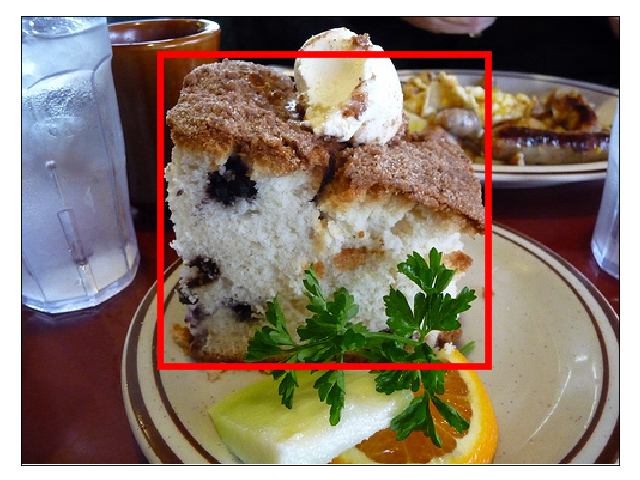
\includegraphics[scale=0.15]{figures/2390077_1254219_supercat_unique.png} &
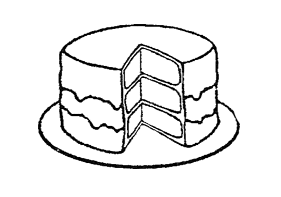
\includegraphics[scale=0.4]{figures/snodgrass_vanderwart_cake_042.png}\\
 cake\ (53),  food\ (19), bread\ (8), burger\ (6), dessert\ (6), snacks\ (3), muffin\ (3),  pastry\ (3) & \hspace{.9cm} cake (83)
\end{tabular}
\caption{Names for a cake object in ManyNames (left) and in cite{snodgrass} (right), percentages of responses in parentheses.}
\label{fig:cake}
\end{figure}


We take a first step at studying natural naming of objects in real-world images and contribute a new dataset, ManyNames, that contains 36 crowd-sourced names for 25K instances from \vg.
Thus, our images show objects in complex visual contexts,
unlike the ``clean'' ImageNet data~\cite{imagenet_cvpr09} that has been previously used to train object classifiers \cite{ILSVRC15}, and unlike stylized line drawings used in picture naming experiments in Cognitive Science (see Figure \ref{fig:cake}).

As illustrated for an object of the class ``cake'' in Figure \ref{fig:cake}, our data reveals clear naming preferences (53\% of the annotators prefer the basic-level \textit{cake}) and also rich variation (the remaining annotators prefer other options like \textit{food, dessert, bread}) which is not restricted to taxonomical relations studied in previous work on naming \cite{rosch1976basic,Ordonez:2016,graf2016animal}.


\section{Background}

\subsection{Object Naming as a Linguistic Phenomenon}

The act of naming an object amounts to that of picking out a nominal to be employed to refer to it (e.g., ``the \refexp{dog}'', ``the white \refexp{dog} to the left'').
Since an object is simultaneously a member of multiple categories (e.g., a young \refexp{beagle} is at once a \cat{dog}, a \cat{beagle}, an \cat{animal}, a \cat{puppy} etc.), all the various names that lexicalize these constitute a valid alternative, meaning that the same object can be named with more or less \textbf{specific names} \cite{brown1958shall,murphy2004big}. 
Seminal work on concepts by Rosch suggests that object names typically exhibit a preferred level of specificity called the \textbf{entry-level}. This typically corresponds to an intermediate level of specificity, i.e., \textbf{basic level} (e.g, \refexp{bird}, \refexp{car}) \cite{rosch1976basic}, as opposed to more generic (i.e., \textbf{super-level}; e.g., \refexp{animal}, \refexp{vehicle}) or specific categories (i.e., \textbf{sub-level}; e.g., \refexp{sparrow}, \refexp{convertible}). However, less prototypical members of basic-level categories tend to be instead identified with sub-level categories (e.g., a \cat{penguin} is typically called a \refexp{penguin} and not a \refexp{bird}) \cite{jolicoeur1984pictures}. 
%This out-of-context preference towards a certain taxonomic level is often referred to as \textbf{lexical availability}. 
While the traditional notion of entry-level categories suggests that objects tend to be named by a \refexp{single} preferred concept, research on pragmatics has found that speakers are flexible in  
%with respect to the chose level of specificity. 
their choice of the level of specificity. 
Scenarios where multiple objects (of the same category) are present induce a pressure for generating names which uniquely identify the target \cite{olson1970language}, such that sub-level names can be systematically elicited in these cases %\cite{rohde2012communicating} \cite{graf2016animal}. 
\cite{rohde2012communicating}\cite{graf2016animal}.
For example, in presence of more than one dog, the name \textsl{dog} is ambiguous and a sub-level category (e.g., \textsl{rottweiler}, \textsl{beagle}) is more informative and potentially preferred by speakers, though additional factors such as cost or saliency also come into play \cite{graf2016animal}\cite{clark1983common}.

\subsection{Visual Object Recognition}

This line of research studies and models object representations in the human visual system, (cf.\ \newcite{regan2000human,rossion2004revisiting}). 
An important experimental paradigm here is picture naming, where subjects have to say or write down the first name that comes to mind when looking at a picture of (typically) a line drawing depicting a prototypical instance of a category \cite{snodgrass}, see Figure\ \ref{fig:cake}.
Subjects reach very high agreement in this task \cite{rossion2004revisiting}, and the resulting naming norms are useful for studying various cognitive processes \cite{humphreys1988cascade}.
Our task is inspired by picture naming, but uses real-world images with objects highlighted in them.
Recognition of instances (as opposed to categories) in images has also been the focus of Computer Vision, where state-of-the-art systems are now able to predict thousands of different categories, (e.g.\ \newcite{googlenet}). 
Current recognition benchmarks use labels (and images) from the ImageNet \cite{imagenet_cvpr09} taxonomy, but typically implement a single ground-truth label approach. 
%, but typically implement multi-label classifiers where relations between labels are not considered \cite{ILSVRC15}. 
%\cs{do you mean multi-label classifiers in single ground-truth label settings?}
In L\&V, deep object recognition systems are widely used for feature extraction, whereas the object labeling itself can often not be used directly. For instance, many labels in the ILSVRC  challenge \cite{ILSVRC15} correspond to very specific breeds of animals, whereas other common categories  for,\ e.g.,\ people are missing.

\subsection{Hierarchical Object Categorization} 
%goes beyond isolated object categories.
% but looks at the principles underlying the organization of object categories. 
... This line of research has emphasized the taxonomic organization of categories, e.g.\ seminal work on prototypes by \newcite{rosch1976basic},  and found that humans tend to conceptualize objects at a basic or medium level of abstraction.
Granularity-aware object recognition methods have incorporated the taxonomic structure underlying object labels in multi-label settings \cite{deng2014large,wang2014poodle,peterson2018learning}, as an account to the criticism on the use of single-labels. 
%While this work goes beyond the simplistic modeling assumption that categories are just unrelated labels, 
%but still aim to predict a single canonical category. % (that does have relations to other categories). 
The purely taxonomic view has been criticized in more recent work on concept organization, which found that many objects of our daily lifes are part of multiple category systems at the same time \cite{ross1999food,SHAFTO20111}. 
This \textit{cross-classification} occurs, for instance, with food categories which can be taxonomy-based (e.g.\  \refexp{meat, vegetable}) or script-based (e.g.\  \refexp{breakfast, snack}).
To the best of our knowledge, this phenomenon has not received any attention in L\&V.
Our results, however, suggest that cross-classification occurs very frequently when naming objects in real-world images.


\subsection{Object Naming in L\&V} 

... work that models which \textit{word} (i.e.\ not label) a speaker will use to name an object is relatively scarce.
Though names are prominent in referring expressions, investigated a lot in natural language generation \cite{dale:1995}, this area has focused mostly on the selection of attributes % rather than on determining the referent's name 
\cite{krahmer:2012}. 
\newcite{Ordonez:2016} takes up the notion of entry-level categories \cite{rosch1976basic} and transfers an object's predicted fine-grained label to its name using text corpus statistics.
% extend object recognition to naming, taking up the notion of entry-level categories \cite{rosch1976basic}.
%Their model predicts classifies objects into fine-grained categories and then predicts a WordNet synset for retrieving the name, based on frequencies in a text corpus. 
 \newcite{zarriess-schlangen:2017} learn a naming model on referring expressions and real-world images, but focus on combining visual and distributional information. 
 Recent experimental work on reference found that the specificity of a name is dependent on the taxonomic relatedness of other objects in context
\cite{rohde2012communicating,graf2016animal}. Our work is a first step towards studying naming in real-world, natural reference.
But as there is virtually no existing large-scale resource that provides robust naming data elicited from multiple subjects \textit{and} for instances in real-world images, this paper focuses on naming in isolation, rather than reference where naming interacts with attribute selection.




\section{Object Names in Existing L\&V resources}


\subsection{Visual Genome}

\vg \cite{krishna2016visualgenome} is one of the most densely and richly annotated resources currently available in L\&V. In the following, we will focus on describing aspects immediately relevant to object naming only, while many other annotations are available as well (e.g. questions, paragraphs, etc.)

\paragraph{Collection and annotation procedure}

\vg aims to provide a full set of descriptions of the scenes which images depict in order to spur complete scene understanding. 
The data collection followed a complex procedure, involving many different rounds of annotation. The first round of the procedure, and the basic backbone for the further rounds, is a collection of region-based descriptions: workers were asked to describe regions in the image and draw boxes around the corresponding area in the image. In this stage, workers were encouraged to annotate 
In a second independent round (involving new workers), annotators were then asked to process the region descriptions by (i) marking the object names contained in the region description, and (ii) drawing a tight box around the corresponding region. As different region descriptions would potentially mention the same objects, each worker was shown a list of previously marked objects and encouraged to select on existing object rather than annotating a new one.


\begin{figure}
\begin{center}
%\fbox{\parbox{6cm}{
%This is a figure with a caption.}}
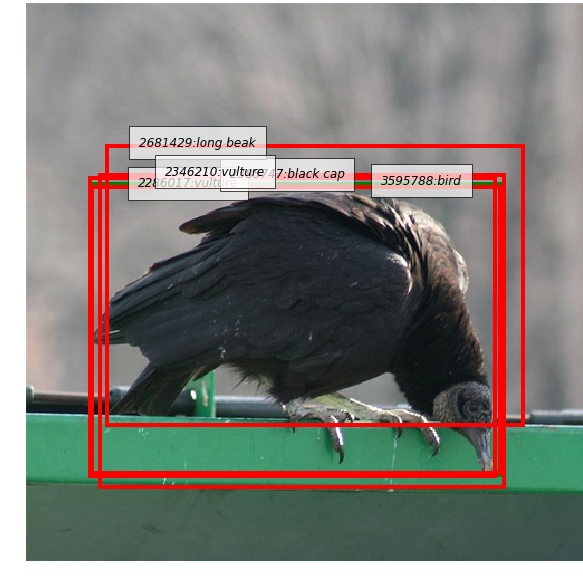
\includegraphics[scale=0.4]{figures/vulture.png} 
\begin{tabular}{lp{6cm}}
object id & linked region descriptions\\
\hline
3595788 & the \textbf{bird} is black in color, nose of the \textbf{bird}, a \textbf{bird} relaxing in stand, small white beak of \textbf{bird}, large black talon of \textbf{bird}, a \textbf{bird} on a green pole, a green bar under \textbf{bird}, black \textbf{bird} on green rail, small black eye of \textbf{bird}\\
2286017 & large black \textbf{vulture} on fence, a vulture on bar\\
2385747 & small white beak of \textbf{bird}\\
2681429 & a semi \textbf{long beak}\\  
2346210 & a black and gray \textbf{vulture}\\
 \end{tabular}
\caption{Bounding boxes, names and region descriptions for an object in VisualGenome}
\label{fig:bird}
\end{center}
\end{figure}

\paragraph{Example}

Figure \ref{fig:bird} shows an example image from VisualGenome, and some of its object annotations. This illustrates that there is only a partial linking of objects that are mentioned across different region descriptions, i.e.\ the identity of objects cannot be established based on the annotation. for a given object and its bounding box, there might be different region descriptions and names associated with it.

\paragraph{Discussion}
\begin{itemize}
\item advantages: exhaustive annotations of all/most objects in the image, variable region descriptions and possibly object names
\item disadvantages: object linking is partial due to bottom-up annotation procedure
\end{itemize}

\subsection{\refcoco and \refcocop}
Both datasets use the \referit\cite{Kazemzadeh2014} game for collecting referring expressions (RE) for natural objects in real-world images, and are built on top of the MS COCO \cite{mscoco}, 
%The latter provides five captions for each of  $300k$~images, spanning $80$~of the COCO categories.  
%However, the COCO region-level (object) annotations are not linked to the captions.
a dataset of images of natural scenes of $91$~common object categories (e.g.,~\cat{dog, pizza, chair}). 
The REs were collected via crowdsourcing in a two-player reference game designed to obtain REs uniquely referring to the target object. 
Specifically, a director and a matcher are presented with an image, and the director produces a RE for an outlined target object in the image. 
The matcher must click on the object he thinks the RE refers to. % (For more details on the datasets see \cite{Yu2016}). 
REs in \refcoco/+ were collected under the constraints that (i) all images contain at least two objects of the same category (80 COCO categories), which prompts the players to avoid the mere object category as RE, and (ii) in \refcocop the players must not use location words, urging them to refer to the appearance of objects. 
%Another critical property of the data is that, (iii), not all objects in an image were annotated with REs, may it due to the frequency constraint~(i), or due to the object not being part of the 80 COCO categories. 

\begin{itemize}
     		\item[(1)] \textbf{Specific categories}: not available, the $80$~COCO categories tend to be entry-level categories and are not linked to the ImageNet taxonomy (e.g.,~\cat{bird, person, car, bus})
		\item[(2)] \textbf{Exhaustive annotations}: not available, as not all objects were annotated with REs and corresponding categories
		   \item[(3)] \textbf{Natural names}: available, though it is unclear how the additional constraints in RefCoco+ impact on the naturalness of object naming
\end{itemize}

\paragraph{Analysis} We parse REs in \refcoco with the Stanford Dependency Parser and extract the nominal heads. We map these names to their most frequent sense/synset in WordNet.
We hypothesize that the distance of a name's synset to the root node (\cat{entity}) relates to its specificity.
We estimate this distance as the minimal path length of all synsets of a word  to the root node.
Table \ref{tab:specnames} shows the estimated levels of specificity for object names in the \refcoco data set.
We observe distances to the root between 2 and 17, meaning that there is a much more fine-grained distinction of levels than the three-way classification adopted in \cite{graf2016animal}.
Unfortunately, the levels of specificity predicted by WordNet do not seem to reflect linguistic intuitions, e.g.\ \refexp{elephant} is predicted to be more specific than \refexp{panda}.
At the same time, this overview clearly suggests that object names in \refcoco do not only comprise entry-level categories, but also very general (\refexp{thing}) and very specific names (\refexp{ox}).

\begin{table*}
\centering
\setlength{\tabcolsep}{2pt}
\begin{small}
\begin{tabular}{rrl|rrl}
\toprule
 spec. &  rel.freq. &                          top 5 names & spec. &  rel.freq. &                          top 5 names \\
\midrule
           2 &   $<$ 0.01 &       \tiny                  thing,things & 10 &   0.05 &   elephant,couch,truck,vase,suitcase \\
           3 &   $<$ 0.01 &    object,group,set,substance,objects & 11 &   $<$ 0.01 &    motorcycle,clock,mom,dad,scissors \\
           4 &   0.14 &           man,person,piece,head,part & 12 &   $<$ 0.01 &  oven,airplane,suv,taxi,refrigerator  \\
           5 &   0.10 &       player,glass,baby,front,corner & 13 &   $<$ 0.01 &    laptop,fridge,canoe,orioles,pigeon \\
           6 &   0.21 &              woman,girl,kid,boy,bowl & 14 &   $<$ 0.01 &   panda,freezer,penguin,rooster,rhino \\
           7 &   0.25 &            guy,right,chair,lady,bear & 15 &   0.03 &    zebra,giraffe,zebras,giraffes,deer \\
           8 &   0.11 &           horse,bus,cow,pizza,batter & 16 &  $ <$ 0.01 &       bison,mooses,orang,elks,sambar \\
           9 &   0.09 &         shirt,car,bike,donut,catcher & 17 &   $<$ 0.01 &           ox,cattle,gnu,mustang,orca \\          
\bottomrule
\end{tabular}\caption{Levels of specificity for naming choices in RefCOCO: for each level (distance between name and WordNet root), relative frequency and 5 most frequent names are shown}
\label{tab:specnames}
\end{small}
\label{tab:specnames}
\end{table*}


\subsection{Flickr30k Entities}
The \flickr dataset \cite{plummer2015flickr30kentities}\footnote{Available at  \url{web.engr.illinois.edu/~bplumme2/Flickr30kEntities}}  augments Flickr30k, a dataset of 30k~images and five sentence-level captions for each of the images, with region-level annotations. 
Specifically, mentions of the same entities across the five captions of an image are linked to the bounding boxes of the objects they refer to. 
The dataset was designed to advance image description generation and phrase localization in particular (e.g.,~\cite{rohrbach2016grounding,plummer2017phrase,yeh2018unsupervised}). 

By design, \flickr can be used to study the way people refer to individual entities in an image depending on the situation the speakers describe and,  
in contrast to \refcoco/+, the production of entity mentions did not underlie any constraints. 
On the other hand, it is less suited for referring expression generation since mentions in isolation of their linguistic context may not uniquely identify the referred object. 

\begin{itemize}
     		\item[(1)] \textbf{Specific categories}: are not available, object categories tend to be even less specific than those of COCO (e.g.,~\cat{people, animals, bodyparts, clothing}), or are abstract (\cat{other, scene})
		\item[(2)] \textbf{Exhaustive annotations}: are not available
		   \item[(3)] \textbf{Natural names}: are available, though object names might not be fully discriminative (as in REs; e.g.,~both animals in the right-most image in Fig.~\ref{fig:graf_genome} are named \refexp{dog})

\end{itemize}

\section{A New Dataset: Many Names}
	\label{sec:data}
	% Number of images/objects:        25,596\\
% Number of object names:  450\\
% Number of collection nodes (synsets):    52 \\

\begin{table*}[htp]
	\small
	\centering
	\begin{tabular}{lp{14cm}}
			\toprule
			Domain & \multicolumn{1}{c}{Collection synsets}\\
			\midrule			
			animals\_plants & ungulate$_1$ (2037), horse$_1$ (833), feline$_1$ (763), dog$_1$ (688)
			bird$_1$ (389), flower$_1$ (44), rodent$_1$ (27), insect$_1$ (12), fish$_1$ (11)\\
			buildings      &  house$_1$ (364), bridge$_1$ (297), shelter$_1$ (169), restaurant$_1$ (58),
                                         outbuilding$_1$ (31), hotel$_1$ (19), housing$_1$ (17), place\_of\_worship$_1$ (12)     \\
			clothing       &  shirt$_1$ (968), overgarment$_1$ (786), dress$_1$ (199), headdress$_1$ (135),
                                         neckwear$_1$ (65), robe$_1$ (27), glove$_2$ (7), footwear$_1$ (5)    \\
			food           &  dish$_2$ (812), baked\_goods$_1$ (770), foodstuff$_2$ (280), vegetable$_1$ (48),
                                         edible\_fruit$_1$ (42), beverage$_1$ (23)   \\
			home           &  furnishing$_2$ (5,355), vessel$_3$ (525), kitchen\_utensil$_1$ (132), crockery$_1$ (92),
			cutlery$_2$ (82), tool$_1$ (72), lamp$_1$ (34)    \\
			people         & woman$_1$ (1768), man$_1$ (1167), male\_child$_1$ (853), athlete$_1$ (396),
			 child$_1$ (333), creator$_2$ (11), professional$_1$ (5)    \\
			vehicles       &  aircraft$_1$ (1208), train$_1$ (957), car$_1$ (727), motorcycle$_1$ (564),
                                         truck$_1$ (559), boat$_1$ (499), ship$_1$ (38)    \\
			\bottomrule
		\end{tabular}
		\caption{Overview of the ManyNames dataset: Synset nodes for each domain (subscript indicates synset number; number of instances in parentheses).
                  \label{tab:overview_dataset2}}
	\end{table*}

\begin{table*}[htp]
	\small
	\centering
	\begin{tabular}{@{~}l@{~}l@{~}l@{~}l@{~}l@{~}l@{~}l}
		\toprule
		vehicles &            food & animals\_plants &           home &        buildings &             people &      clothing \\
		\midrule
		train (954) &  pizza (518) &  giraffe (915) &  bed (888) &  house (340) &  boy (853) &  shirt (904) \\
		car (642) &  cake (261) &  horse (822) &  bench (714) &  bridge (274) &  man (806) &  jacket (451) \\
		plane (485) &  bread (186) &  cat (754) &  table (687) &  dugout (91) &  woman (766) &  coat (267) \\
		airplane (479) &  sandwich (153) &  dog (654) &  desk (672) &  tent (53) &  girl (650) &  dress (190) \\
		motorcycle (466) &  bun (143) &  zebra (461) &  counter (516) &  restaurant (33) &  lady (342) &  hat (77) \\
		% truck (465) &  cheese (110) &  cow (324) &  couch (366) &  overpass (23) &  guy (330) &  t-shirt (62) \\
		% boat (450) &  donut (78) &  bird (295) &  chair (365) &  grill (22) &  child (230) &  tie (51) \\
		% jet (106) &  salad (70) &  sheep (216) &  carpet (307) &  garage (18) &  batter (110) &  blazer (43) \\
		% aircraft (85) &  sauce (68) &  bull (48) &  bowl (219) &  hotel (16) &  kid (85) &  hood (26) \\
		% van (76) &  apple (33) &  flower (40) &  curtain (182) &  castle (14) &  skateboarder (80) &  cap (20) \\
		\bottomrule
	\end{tabular}
	\caption{Overview of the ManyNames dataset: Top 5 VG names for each domain (number of instances in parentheses).\label{tab:overview_dataset1}}
\end{table*}

\begin{figure*}[htp]
  \centering
  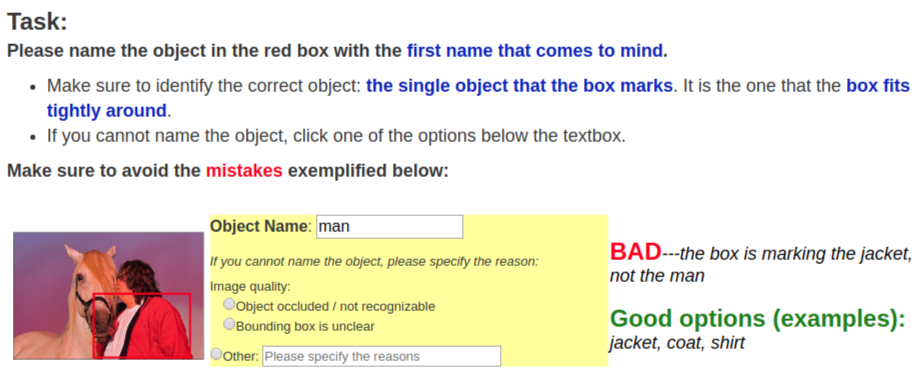
\includegraphics[width=1.5\columnwidth]{figures/round0_cropped.png}
  \caption{Instructions for AMT annotators for the first round (whole instructions showed more examples, see Figure~\ref{fig:instructions2}).}
  \label{fig:instructions1}
\end{figure*}

We take data from \vgenome~(VG, \newcite{krishna2016visualgenome}), which
contains a dense region-based labeling of $108$K~images with, inter alia, object names, attributes and relationships,
all linked to WordNet synsets \cite{fellbaum1998wordnet}.
\vg suits our purpose of collecting names for naturalistic instances of common objects, as it has images of varying complexity, with close-ups as well as images with many objects.
As common in Computer Vision, objects are localized as bounding boxes, as in Figure~\ref{fig:cake}.% 
\footnote{We use image and object interchangeably in the following, since we only selected one target object per image (i.e., each object and image in VG is chosen at most once).}

\subsection{Sampling of Instances}
\label{ssec:sampling}

%Criteria: From CV: select images depicting objects with relatively frequent names; From CogSci: select objects which have been frequently studied in cognitive science/psychological norming studies; we chose McRae et al. as basis.
We selected images from seven domains: \domain{animals\_plants}, \domain{buildings}, \domain{clothing}, \domain{food}, \domain{home}, \domain{people}, \domain{vehicles}. 
They are all based on McRae et al.'s  \cite{mcrae2005semantic} feature norms, a dataset widely used in Psycholinguistics that comprises common objects of different categories, except for \domain{people}, which we added because it is a very frequent category in \vg and a very prominent category for humans.
% We start from the concepts of McRae et al.'s feature norms (REF), which are common objects of different categories (e.g.,~\domain{animals}, \domain{furniture}) and, as such, have a high overlap with standard datasets of object norming studies (REFS).
% We added the \domain{person} category because it is very frequent category in \vgenome.

Within each domain, we aimed at collecting instances at different taxonomic levels to cover a wide range of phenomena, but this is not straightforward because ontological taxonomies do not align well with the lexicon (for instance, \textit{dog} and \textit{cow} are both mammals, but \textit{dog} has many more common subcategories), and most domains are not organized in a clear taxonomy in the first place (e.g.\ \domain{home}).
Instead, we defined a set of synsets ($52$\ in total; listed in Table~\ref{tab:overview_dataset2}) that we used to collect object instances from \vg, as follows. 

First, to create our synset set, we chose those \vg synsets that match or subsume the object classes in the McRae norms, and have a high number of \vg object instances of different names.\cs{prev. sentence this is still a bit fluffy}
For example, \vg instances subsumed by McRae's \textsl{dog} were named \textsl{beagle, greyhound, puppy, bulldog}, etc., while McRae's \textsl{duck}, \textsl{goose}, or \textsl{gull} did not have name variants in \vg, so we kept \textsl{dog} and \textsl{bird} (which subsumes \textsl{duck}, \textsl{goose}, or \textsl{gull}) as collection synsets.
%\gbt{Just to clarify: we also collected objects named \textsl{duck}, \textsl{goose}, or \textsl{gull}, right? Not only \textsl{bird}?}

We then retrieved all VG images depicting an object whose name matches or is subsumed by words in one of these synsets; we refer to these words as \textit{seeds} ($450$\ in total).
\gbt{from the dataframe in the github it's 449. Also, there are some mistakes in the list of seeds ('dugout.', 'man's') -- to check after the deadline.}
We did not consider objects with names in plural form, with parts-of-speech other than nouns\footnote{We obtained tags with CoreNLP \cite{manning2014stanford}.}, or that were multi-word expressions (e.g.,~\textsl{pink bird}). 
We further only considered objects whose bounding box covered~\mbox{$20-90\%$} of the image area.
% We based the definition of our set of nodes on the WN (REF) synsets of the McRae concepts (e.g.,~dog, duck, goose, gull), the nominal WordNet hierarchy, and the frequency distribution of the VG object names' synsets.\footnote{TODO: need to be clear from the general description of VG that the frequ. of instances labeled with the synset of the object name is meant.} 
% First, we selected a set of collection node candidates---synsets which match (e.g.,~\textsl{dog, duck, goose, gull}) or subsume (e.g.,~\textsl{mammal, bird}) the McRae synsets\footnote{Specific synset IDs, e.g.,~dog.n.01, are omitted for readability.}. 
% From these candidates we kept those as collection nodes which had a high frequency of VG object instances of different names. For example, VG instances  subsumed by McRae's \textsl{dog} were named \textsl{beagle, greyhound, puppy, bulldog}, etc., while McRae's \textsl{duck, goose}, or \textsl{gull} did not have name variants in VG, so we kept \textsl{dog} and \textsl{bird} as collection nodes.
%\paragraph{Collection of instance candidates}
% Goal of above procedure was the collection of instances of selected object classes---our nodes--- whose VG names correspond to or subsume (are hypernyms of) a McRae concept, and whose object names differ, that is, of which we can expect that people possess different names for them (e.g.,~\textsl{duck, goose, gull} for \textsl{bird}).
% \paragraph{Sampling of instances}
Because of the Zipfian distribution of names, and to balance the collection, we sampled instances depending on the size of the seeds: up to $500$\ instances for seeds with up to $800$\ objects, and up to $1000$\ instances for larger seeds. This yielded a dataset of\ $31,093$~instances, which was further pruned during annotation, as explained next.
Table~\ref{tab:overview_dataset1} shows the top 5 \vg names in each of the domains.

\subsection{Elicitation Procedure}
\label{ssec:elicitation}

To elicit object names, we set up a crowdsourcing task on Amazon Mechanical Turk (AMT).
In initial pilot studies, we found object identification via bounding boxes to be problematic.
In some cases, the bounding box was not clear; in others, AMT workers named objects that were more salient than the one signaled by the box (for instance, for a box around a jacket, the man wearing it).
We took special care of minimizing this issue in two ways: Specifying the instructions such that workers pay close attention to what object is being indicated in the box, and pruning images with unclear boxes or occluded objects via an initial collection round in which we allowed workers to mark such cases.
Figure~\ref{fig:instructions1} shows the task instructions for this first round, in which 9 workers annotated each image.

%We eliminated around $5.5$K\ images based on pruning, obtaining the final dataset with $25,596$\ images.
After the first round, and based on the opt-out annotation, we kept images that met all the following conditions (thresholds were estimated via manual inspection): (i) they were not marked as occluded by any subject; (ii) ``Bounding box is unclear'' was marked at most twice; (iii) at most 17\% of elicited names were in plural form (to remove cases where the bounding box contains several objects); (iv) the most frequent elicited name is of the same domain as the \vg name.
This yielded $25,596$ images (we discarded $5,497$).
We then did 3 more collection rounds, obtaining a total of 36 images per object.
Figure~\ref{fig:instructions2} shows the instructions for these rounds; they were accompanied by a FAQ solving common issues. 
We shuffled the set of images per task between rounds, and workers could only participate in one round, to avoid workers annotating an instance more than once.
Overall $841$\ workers took part in the data elicitation, with a median of  $261$\ instances \mbox{($\textrm{range}=[9,17K]$)} per worker.

\begin{figure*}[htp]
  \centering
  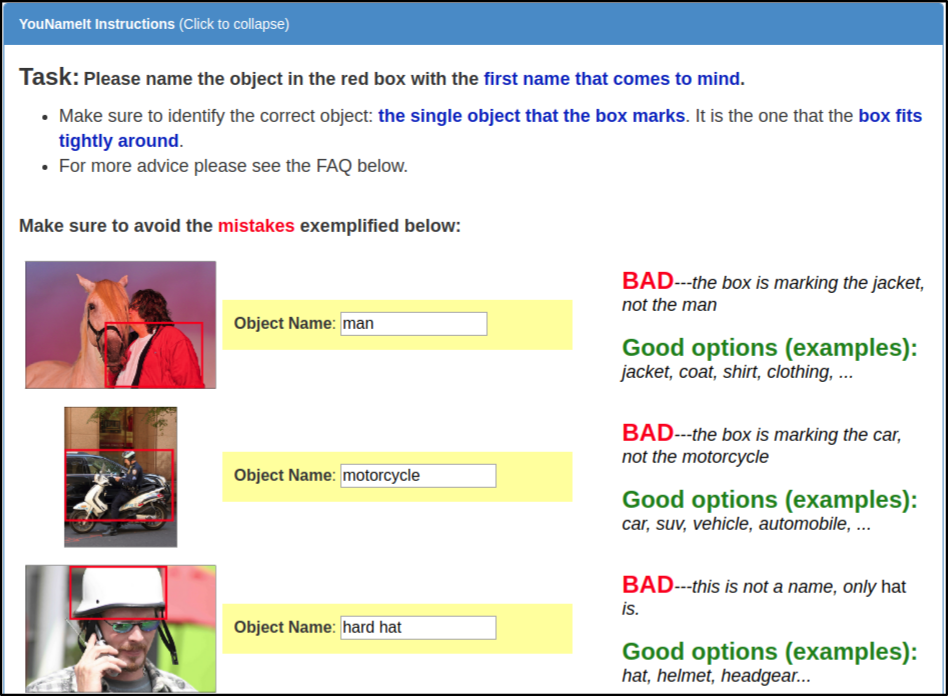
\includegraphics[width=1.5\columnwidth]{figures/round1+_p1.png}
  \caption{Instructions for AMT annotators for rounds~$2$ to~$4$.}% They were accompanied by the FAQ in Figure~\ref{fig:faq}}
  \label{fig:instructions2}
\end{figure*}

% \begin{figure*}[htp]
%   \centering
%   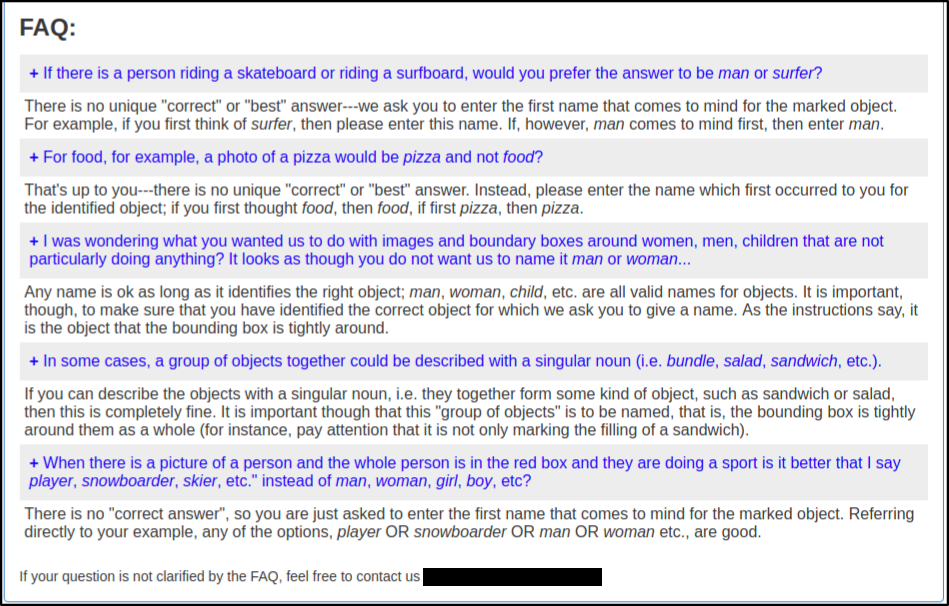
\includegraphics[width=1.5\columnwidth]{figures/round1+_p2.png}
%   \caption{FAQ accompanying the instructions for AMT annotators for rounds~$2$ to~$4$.}
%   \label{fig:faq}
% \end{figure*}

%\cs{Maybe say something about the rejections, if space permits it.}

%%% Local Variables:
%%% mode: latex
%%% TeX-master: "lrec2020naming"
%%% End:



	
	\section{Analysis}
	\label{sec:analysis}
	%\gbt{Points to discuss in the paper, as discussed with Carina May 16:}
%
%\begin{itemize}
%\item Super high variance in the agreement. Higher agreement for instances, lower for classes. Suggests systematicities at the instance level that do not depend on the class. Hypothesis, supported by qualitative analysis (Figure 3): relevance of visual perceptual factors. E.g.: saliency, background/foreground (desk-keyboard; bridge-train); ``angle'' from which the object is shown (see girl-t-shirt example); \dots In addition, we also find aspects discussed by Psycholing, but at the level of the instance: Typicality (see truck-bus example, bridge-dock, bench-seat). 
%\item Forget about WordNet.
%\item Implications for lang\&vision: 1) synset classification won't do (if the goal is to predict/label an object); 2) name classification won't do either; 3) ``mistakes'' done by models are also done by humans -- role of referential uncertainty.
%\end{itemize}


In this section, we investigate to what extent names annotated in VisualGenome and elicited in ManyNames can be considered canonical, i.e. to what extent speakers agree in their naming choices.
Whereas traditional picture naming studies typically use a prototypical image per category (see Figure~\ref{fig:picture_naming}) and, hence, are mostly interested in the agreement on concept or category-level, we carry out an analysis on two different levels: First, we will look at instances and see to what extent names overlap for the same object. 
Second, we will use the existing annotation of names in VisualGenome to analyze agreement on the level of classes.
\begin{figure}[t]
	\centering
	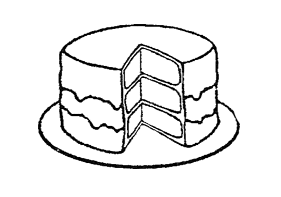
\includegraphics[scale=.5]{figures/snodgrass_vanderwart_cake_042.png}
	\caption{Example of a picture of \textsl{cake} used in traditional picture naming studies (REF to Vanderwart \& Snodgrass) \label{fig:picture_naming}}
\end{figure}

\subsection{Names, instances, classes}

First of all, to see whether objects in ManyNames bear a canonical name, we simply count how many different names (i.e.\ types) are given to instances, and to all instances that have the same synset annotated in VisualGenome. 
As the data is collected via crowdsourcing and a certain amount of noise is to be expected, we apply different frequency thresholds on the response sets for instances and synsets.
Figure \ref{fig:ntypes} shows the cumulative histograms for type counts, obtained with different thresholds (from 1 to 6).
Without any frequency thresholding, the proportion of instances and classes that have a single name annotated is small, i.e.\ below 10\% in both cases. When raising the threshold up to a minimum of 4 occurences in the response set  for instances (meaning more than 10\% of the 36 annotations), the proportion of objects that really only have a single name annotated is considerably higher, but still below 50\%.
Thus, as expected in a free annotation scenario, the MN data contains a certain number of low-frequency responses.
The fact that even after applying a relatively strict frequency filter most objects have more than one name annotated indicates that there is a non-negligible  level of variation when different speakers name the same object.

The amount of variation increases substantially when looking at the number of names we find for different synsets in Visual Genome, as is indicated by the histogram for type counts of synsets in Figure \ref{fig:ntypes}.
Here, we observe that the rise of the curve is much less steep than for instances and, generally, there are many synsets with more than 10 or even 20 different name types, even after applying the frequency threshols.

\begin{figure*}
\begin{minipage}[b]{0.4\linewidth}
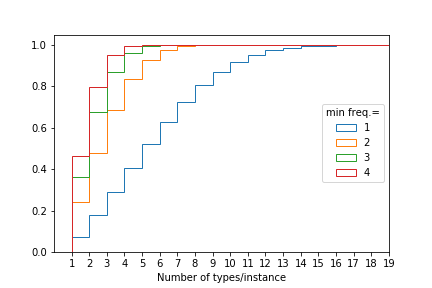
\includegraphics[scale=.4]{Figures/types_instances.png}
\end{minipage}
\begin{minipage}[b]{0.6\linewidth}
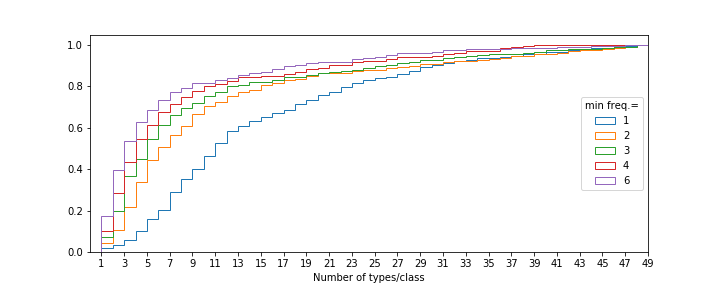
\includegraphics[scale=.4]{Figures/types_classes.png}
\end{minipage}
 \caption{\label{fig:ntypes} Cumulative histograms for number of types found for instances and classes, based on different frequency tresholds (applied on the level of instances and classes respectively)}
\end{figure*}


\subsection{Agreement}

We compute the following agreement measures:

\begin{itemize}
\item \textbf{\% top}: the average relative frequency of the most frequent response (shown in percent)
\item \textbf{$H$}: the $H$ agreement measure used previously in the psycholinguistic literature
\cs{How is this defined?}
\begin{equation}
H = \sum_{i=1}^k p_i\ log_2(1/p_i)
\end{equation}

\item \textbf{N}: the average number of types in the response set of ManyNames
%\item \textbf{N$_{>1}$}: the average number of types, excluding types that have been annotated only once
\cs{alternatively we could show a plot going from 1 to, let's say, $>10$}
\item \textbf{top=VG}: the proportion of items where the top response in ManyNames corresponds to the VisualGenome name
\item \textbf{\% VG}: the average relative frequency of the VisualGenome name in the response set

\end{itemize}

For measuring \textbf{instance-level agreement}, we consider all names annotated for an object as a response set and then average over these response sets. Furthermore, we compute \textbf{class-level agreement} by merging the response sets for all objects that have the same synset (given for the original VisualGenome name) and compute the measures over these aggregated response sets.
\gbt{@Sina, what are the synsets that you got here? Are they collection nodes, or the synset of the VG name as annotated in VG?}


Table \ref{tab:agree} shows the analysis of the instance-level and category-level agreement.
On the instance-level, our annotators achieve a fair amount of overlap in their object naming choices. 
Thus, for roughly 70\% of our objects (\textbf{std=?}), the most frequent response in ManyNames corresponds to the original VisualGenome name and, similarly, the average frequency of the top response is also 70\%. 
%Generally, this seems to suggest that indeed many objects in our data set have a canonical name. 
\sz{For NLP people, this looks like a good agreement (given that people were free to type what they wanted). For vision people who might think of it as an object labeling task, this would be pretty low/bad agreement.}
At the same time, the average number of name types per object (5.7, or 2.9 when excluding low-frequency types in each response set) suggests that there is a stable amount of naming variants that is elicited for instances. 
Furthermore, the agreement varies quite considerably among domains \cs{refer to std}:  in the animal domain, which is often discussed in the object naming literature, annotators achieve a very stable and robust agreement of over 90\% and an $H$ agreement which comes close to 0 (where 0 is perfect agreement). 
The people domain, on the other hand, is subject to much more variation and agreement is dramatically lower here, and comes close to 50\% for \% top.



%\gbt{Super-interesting results.}
Finally, the category-level agreement figures tell yet another story: when aggregating the responses for all objects with the same VisualGenome synset, we obtain on average 30 types (with $N_{>1})$, i.e. variants of the original VG class. 
Surprisingly, here, only 32.7\% of the aggregated response sets still have the VG name as the most frequent response, which means that for 70\% of the VG names, annotators in ManyNames, on average, prefer a different name.  
Likewise, the relative frequency of the top response drops considerably and $H$ increases from 1.3 for instance-level agreement to 2.4 on object-level agreement.  
%\cs{Can we say more about what's going on in the people and vehicles domain, category-level, top=VG? E.g., put corresponding examples in Tab.\ref{tab:qual}}
%

\subsection{Variation and WordNet}

Previous work on large-scale collections of labels or names of objects has (explicitly or implicitly) assumed that once naming data is canonical, linguistic alternatives of the canonical name can simply be retrieved from existing taxonomies like e.g.\ WordNet. 
%If this was indeed the case, it would be feasible (and probably even desirable) to canonicalize object names during dataset collection, without loosing too much information about linguistic variations in natural object naming scenarios (like e.g.\ referring expression generation).
Hence, in this section, we investigate to what extent the variation in object naming that we find in our MN data set (see previous Section) is covered by WordNet.
%In this section, we take a closer look at the lexical variation we observe in our data set. 
We analyze the data points where participants attributed different names to the same object and extract a set of  pairwise \textbf{naming variants}. These naming variants correspond to pairs of words that can be used interchangeably to name certain objects.
For each object, we extract the set of naming variants $s = \{ (w_{top},w_2), (w_{top},w_3), (w_{top},w_4),... \}$  where $w_{top}$ is the most frequent name annotated for the object and $w_2 ... w_n$ constitute the less frequent alternatives of $w_{top}$.  The  \textbf{type frequency} of a naming variant $(w_{top},w_x)$ corresponds to the number of objects where this variant occurs. The \textbf{token frequency} of $(w_{top},w_x)$ corresponds the count of all annotations where $w_x$ has been used instead of $w_{top}$.
In Table \ref{tab:exvariants}, we show the naming variants with the highest raw token frequency for each domain. 
The naming variants can be grouped according to their lexical relation, as follows:

\begin{itemize}
\item \textbf{synonymy}: e.g.\ aircraft vs. airplane 
\item \textbf{hyponymy}: e.g.\ man vs. person
\item \textbf{co-hyponymy}: e.g.\ swan vs. goose
\item \textbf{no relation}: e.g.\  desk vs. apple
\end{itemize}

\begin{table}
\small
\centering
\begin{tabular}{lcc}
\toprule
         relation & \% types & \% token \\
\midrule
% meronym &  0.1 &  0.2 \\
% holonym &  0.1 &  0.4 \\
 synonym &  1.1 &  1.1 \\
 hyponym &  2.2 &  3.8 \\
 co-hyponym &  3.1 &  5.9 \\
 hypernym &  10.5 &  27.7 \\
 word-not-covered &  10.6 &  2.6 \\
 rel-not-covered &  72.2 &  58.3 \\
\bottomrule
\end{tabular}
\caption{Lexical relations of naming variants in MN to annotated VG synset, averaged over synsets}
\label{tab:rel}
\end{table}


Research on object naming following the idea of entry-level categories has, essentially, exclusively looked at names that stand in a hierarchical relation (i.e.\ hyponymy/hypernymy).

We use WordNet to extract lexical relations between the naming variants in our data set.
Unfortunately, this means that we have to exclude a certain portion of the data as either (i) one of the name is not covered in WordNet, (ii) we cannot find a lexical relation between the two names (see below). Also, we had to be relatively permissive with respect to the definition of hyponymy/co-hyponymy. 
For instance, to analyze \textit{giraffe} as a hyponym of \textit{animal} we have to look at the closure of the hyponyms of \textit{animal} with a depth of 8 (in WordNet).
\sz{should we call this co-hyponymy or co-hierarchical relation?}

\sz{include Table that reports counts of the naming variants, coverage in WordNet etc.} \gbt{I think it'd be best to put the out-of-wordnet info in the Lexical relations table -- this way we have everything in one place.}

Table \ref{tab:rel} shows the distribution of lexical relations for those naming variants that we were able to analyze with WordNet.
Both in terms of their types and token frequency, the naming variants that instantiate a (loose) co-hyponymy relation are by far the most frequent.
\sz{discuss in more detail, discuss: to what extent is this an artefact of WordNet?}
This is really interesting: most research on object naming, to date, has focussed on hyponymy/hypernymy, i.e. variation that relates to hierarchical relations between object names.
Our data suggests that co-hierarchical variation is really important too.



%\subsection{Qualitative Analysis}

%\sz{put qualititative discussion here} Table \ref{tab:qual} shows examples for canonical and non-canonical VG names in our data set, where canonical means that the name was the top response in the aggregated response set in ManyNames.

%\begin{table}
%\small
%\begin{tabular}{lp{4.8cm}r}
%\toprule
%VG name &  top5 MN names &  n$_{obj}$  \\
%\midrule
%\multicolumn{3}{c}{\it Canonical VG names with max agreement in MN}\\
% giraffe &  giraffe (96.8), animal (1.2), zebra (0.4), camel (0.3), pole (0.1) &  915 \\
% zebra &  zebra (96.3), animal (1.0), giraffe (0.9), horse (0.2), microwave (0.2) &  461  \\
% cat &  cat (94.8), animal (0.9), kitten (0.8), dog (0.4), laptop (0.2) &  754\\
%\midrule
%\multicolumn{3}{c}{\it Canonical VG names with min agreement in MN}\\
% booth &  booth (19.3), table (12.3), phone booth (9.8), bench (6.7), building (4.4) &  11 \\
% cabbage &  cabbage (21.4), lettuce (17.0), hotdog (11.9), food (10.7), salad (10.4) &  9 \\
% robe &  robe (22.1), shirt (16.8), jacket (13.3), dress (5.7), clothing (3.2) &  19 \\
%  \midrule
%  \multicolumn{3}{c}{\it Non-canon. VG names with max agreement in MN}\\
% sedan &  car (88.4), wheel (3.1), vehicle (2.3), automobile (1.3), dog (0.8) &  11 \\
% pony &  horse (83.9), pony (9.1), animal (2.9), donkey (1.1), cow (1.1) &  8 \\
% necktie &  tie (81.4), necktie (10.2), shirt (4.6), ties (1.5), jacket (0.5) &  11 \\
% \midrule
%   \multicolumn{3}{c}{\it Non-canon. VG names with min agreement in MN}\\
% shelter &  umbrella (9.7), shelter (8.8), roof (8.0), tent (7.1), building (6.8) &  10 \\
% bath &  shower (13.3), elephant (9.9), birdbath (8.1), water (7.2), trough (7.2) &  10 \\
% vegetable &  food (15.7), broccoli (13.1), sandwich (10.6), salad (9.3), pizza (7.8) &  25 \\
%\bottomrule
%\end{tabular}
%\caption{Examples for VisualGenome (VG) names and their most frequent corresponding responses in ManyNames (MN; percentages shown in brackets). ``Canonical'' means that the VG name is the top name in MN, and non-canonical vice versa.}
%\label{tab:qual}
%\end{table}

\begin{figure*}
\begin{minipage}[b]{0.5\linewidth}
{\footnotesize
\setlength{\tabcolsep}{1pt}
\begin{tabular}{p{4cm}|p{4cm}|p{4cm}|p{4cm}}
%\textbf{desk} &  \raisebox{-\totalheight}{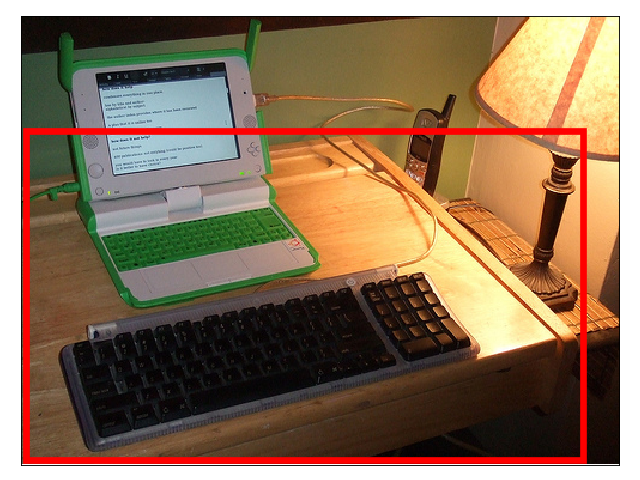
\includegraphics[width=0.9\linewidth]{figures/2320949_1048853_singleton_obj.png}} MN: keyboard  &
%\raisebox{-\totalheight}{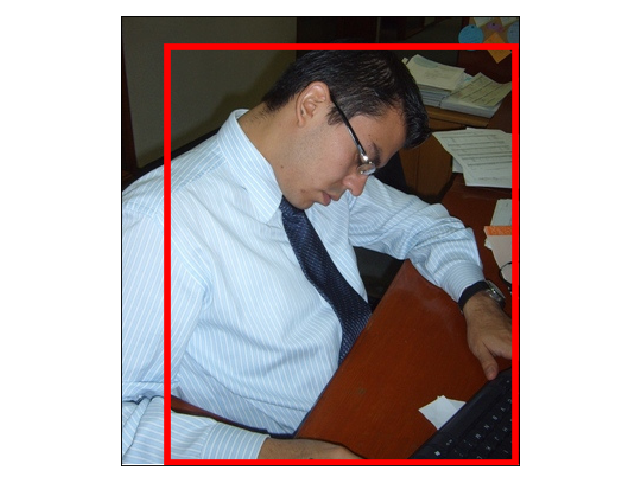
\includegraphics[width=0.9\linewidth]{figures/2343219_926143_supercat_unique.png}}  MN: desktop &
%\raisebox{-\totalheight}{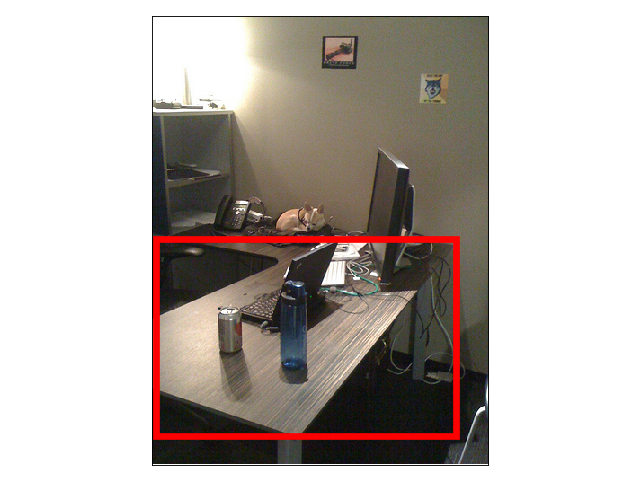
\includegraphics[width=0.9\linewidth]{figures/2354847_1742687_seed_ambiguous.png}} MN: computer \\
%\textbf{bench} &  \raisebox{-\totalheight}{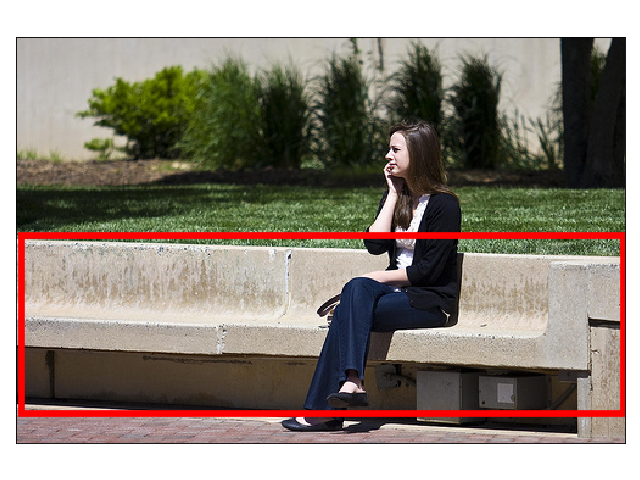
\includegraphics[width=0.9\linewidth]{figures/2350360_1042111_supercat_unique.png}} MN: table  &
%\raisebox{-\totalheight}{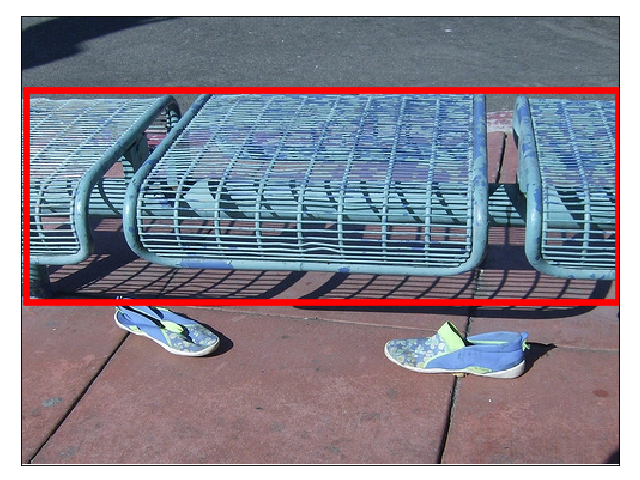
\includegraphics[width=0.9\linewidth]{figures/2389358_1261752_singleton_obj.png}}  MN: seat &
%\raisebox{-\totalheight}{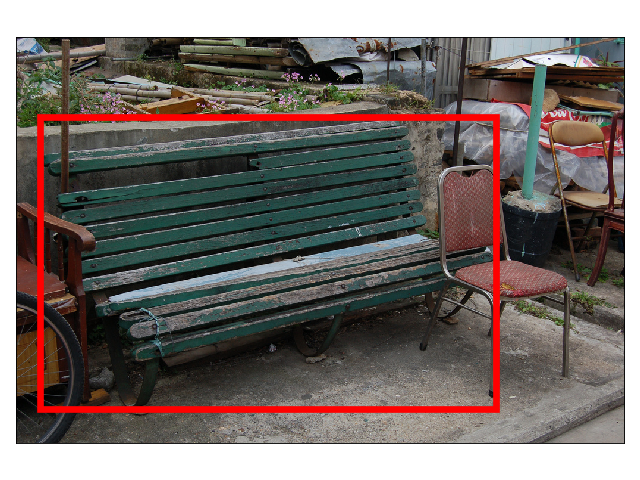
\includegraphics[width=0.9\linewidth]{figures/1593011_2063521_singleton_obj.png}} MN: wood \\
\multicolumn{4}{c}{\textbf{VG: sandwich}}\\
 \raisebox{-\totalheight}{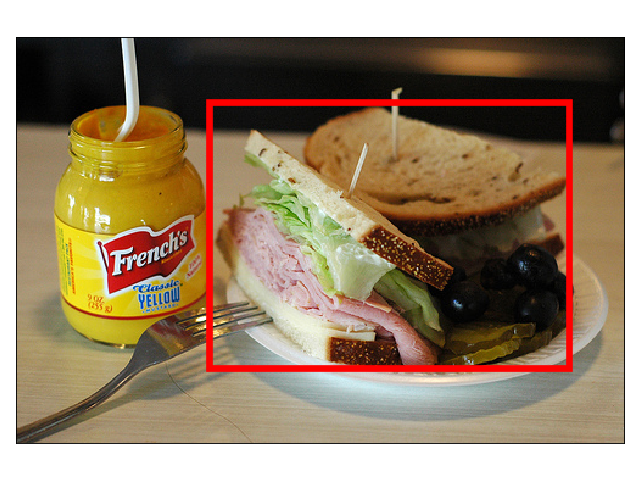
\includegraphics[width=0.9\linewidth]{figures/2339876_3928476_supercat_unique.png}} sandwich (34) &
\raisebox{-\totalheight}{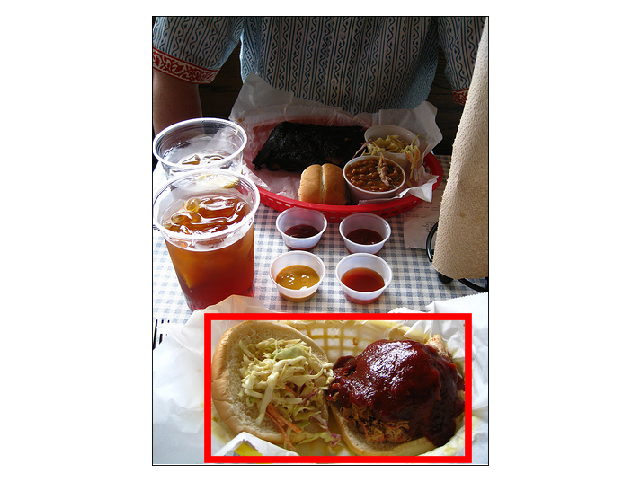
\includegraphics[width=0.9\linewidth]{figures/2379889_1353176_supercat_unique.png}}  sandwich (15), basket (6), food (5), burger (2), hamburger (2), meal (2) &
\raisebox{-\totalheight}{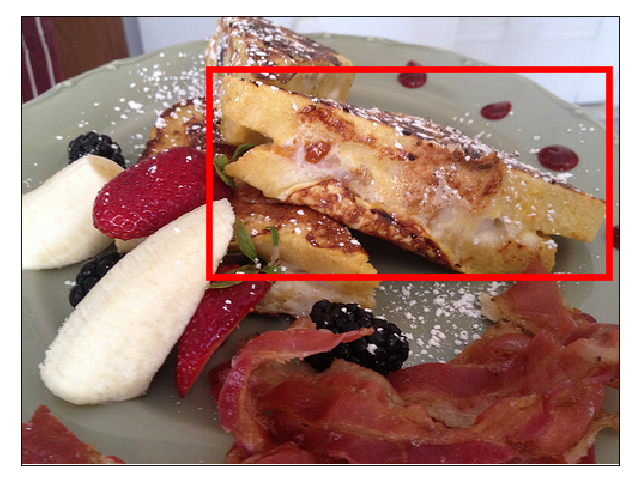
\includegraphics[width=0.9\linewidth]{figures/2394266_465678_singleton_obj.png}} food (10), sandwich (8), toast (5), french toast (4), dessert (2), breakfast (2) &
\raisebox{-\totalheight}{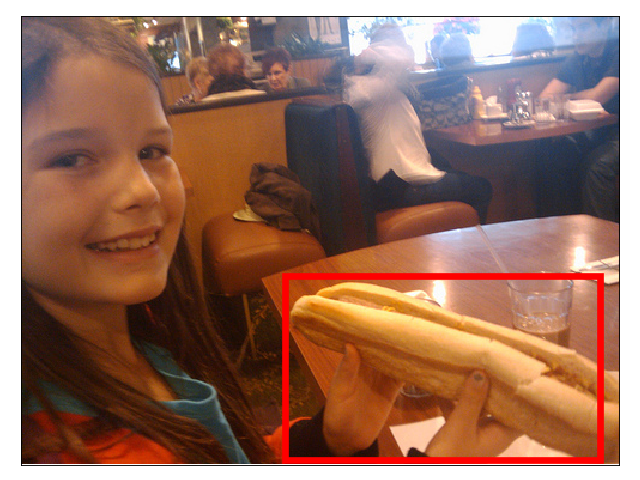
\includegraphics[width=0.9\linewidth]{figures/2386509_681763_supercat_unique.png}} hotdog (14), food (7), bun (4), sandwich (3), bread (2)\\ 
\multicolumn{4}{c}{\textbf{VG: bridge} }\\ 
\raisebox{-\totalheight}{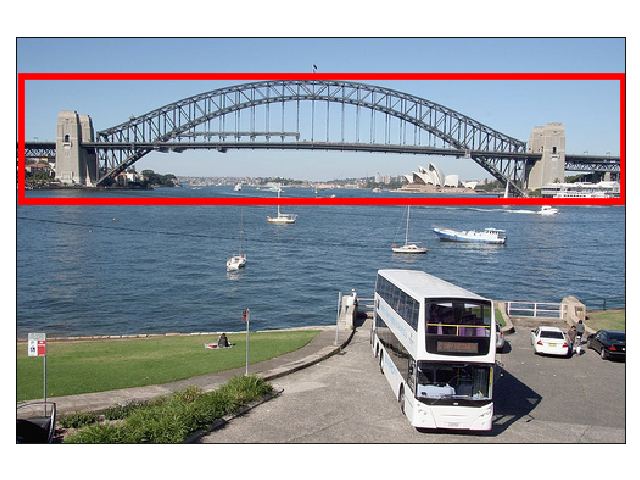
\includegraphics[width=0.9\linewidth]{figures/2341667_2006329_singleton_obj.png}} bridge (35)  &
\raisebox{-\totalheight}{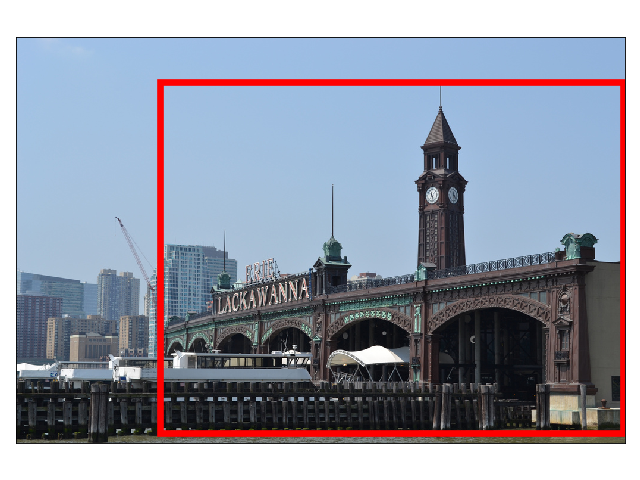
\includegraphics[width=0.9\linewidth]{figures/1592509_1610006_singleton_obj.png}} bridge (20), building (11)  &
\raisebox{-\totalheight}{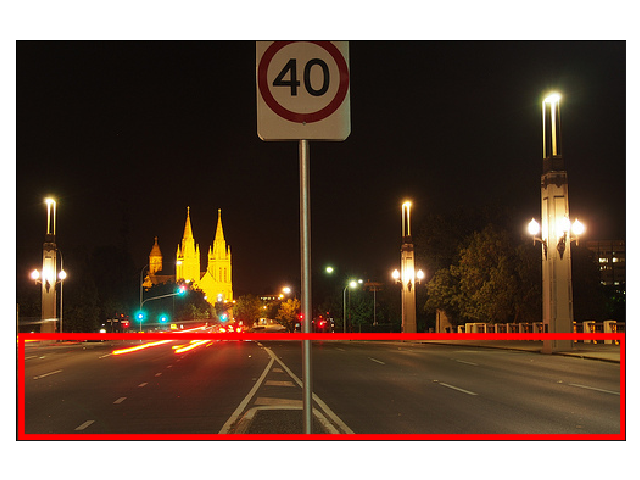
\includegraphics[width=0.9\linewidth]{figures/2384683_1306430_singleton_obj.png}} street (16), road (15), bridge (3) &
\raisebox{-\totalheight}{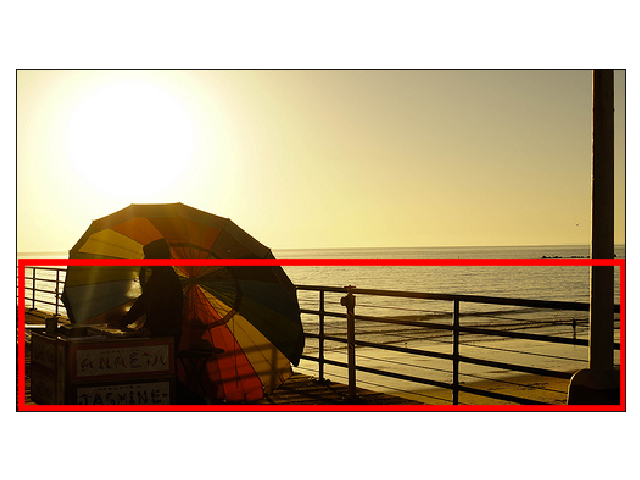
\includegraphics[width=0.9\linewidth]{figures/2412972_3494120_singleton_obj.png}} pier (6), railing (5), dock (5), bridge (5), fence (4), rail (3), boardwalk (3)\\ 
\multicolumn{4}{c}{\textbf{VG: bed}}\\ 
\raisebox{-\totalheight}{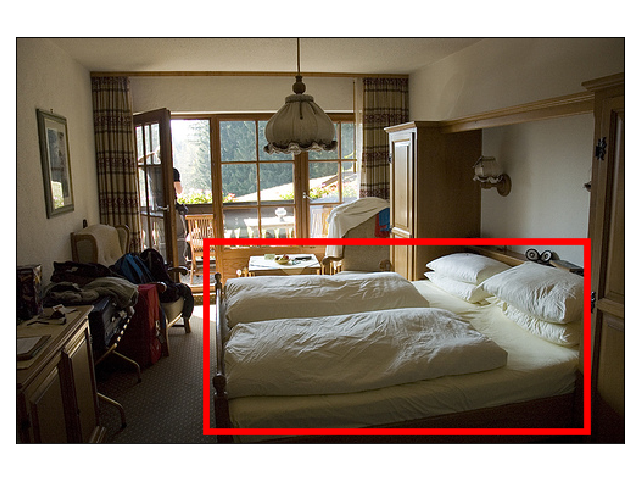
\includegraphics[width=0.9\linewidth]{figures/2321254_3438076_singleton_obj.png}} bed (36)  &
\raisebox{-\totalheight}{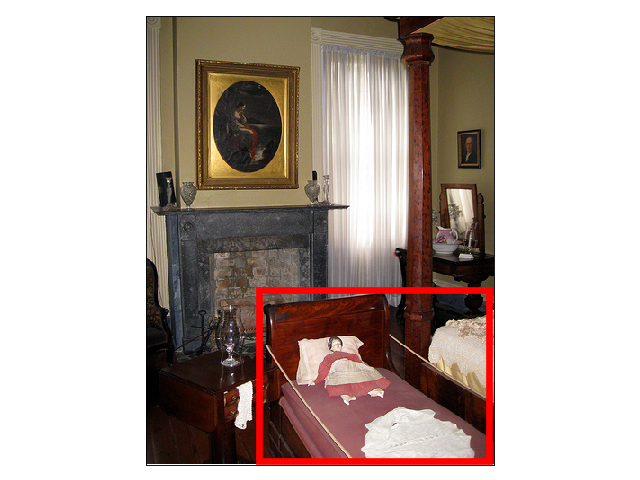
\includegraphics[width=0.9\linewidth]{figures/2324306_3412337_singleton_obj.png}}  bed (16), bench (6), crib (5) &
\raisebox{-\totalheight}{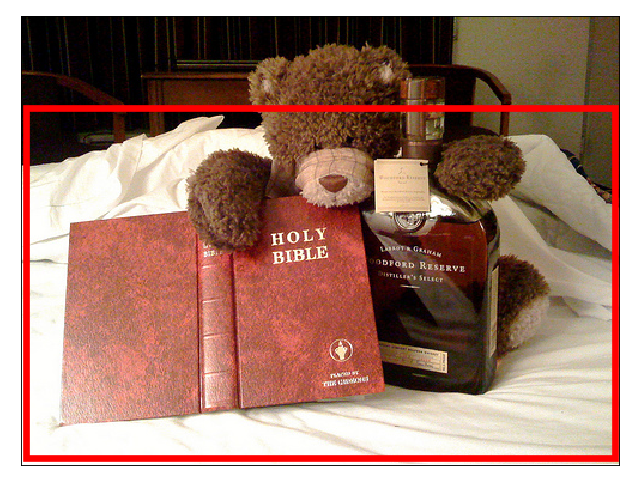
\includegraphics[width=0.9\linewidth]{figures/2342811_3485104_singleton_obj.png}}  bed (17), book (6), table (4), toy (3), bible (2), doll (2) & 
\raisebox{-\totalheight}{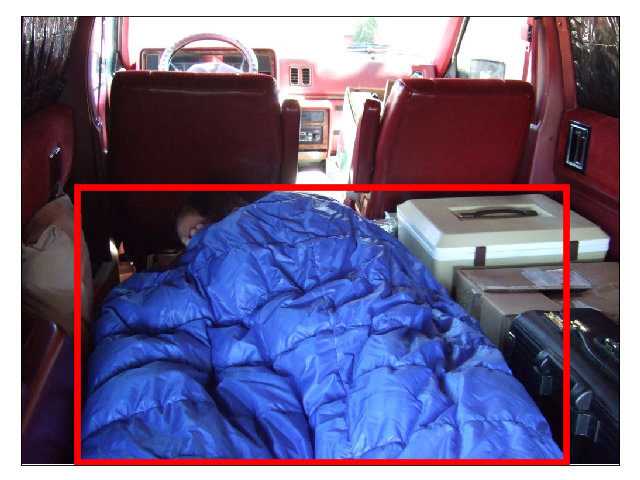
\includegraphics[width=0.9\linewidth]{figures/498222_3135415_singleton_obj.png}} bed (12), sleeping bag (9), blanket (7), bed sheet (5)\\ 
\multicolumn{4}{c}{\textbf{VG: batter}}\\
\raisebox{-\totalheight}{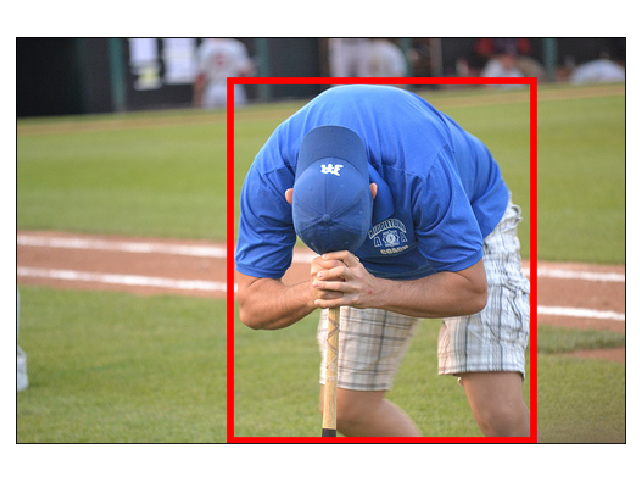
\includegraphics[width=0.9\linewidth]{figures/2372219_2683892_supercat_unique.png}} man (24), cap (5), person (3), baseball player (2) &
  \raisebox{-\totalheight}{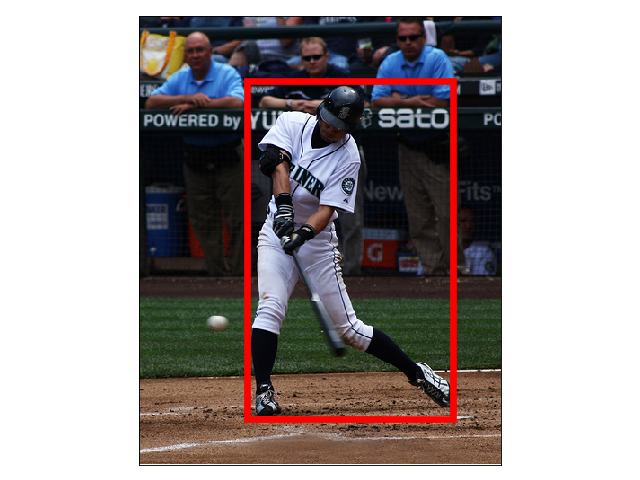
\includegraphics[width=0.9\linewidth]{figures/2394377_464684_singleton_obj.png}} man (13), baseball player (7), batter (5), player (3), helmet (2) &
\raisebox{-\totalheight}{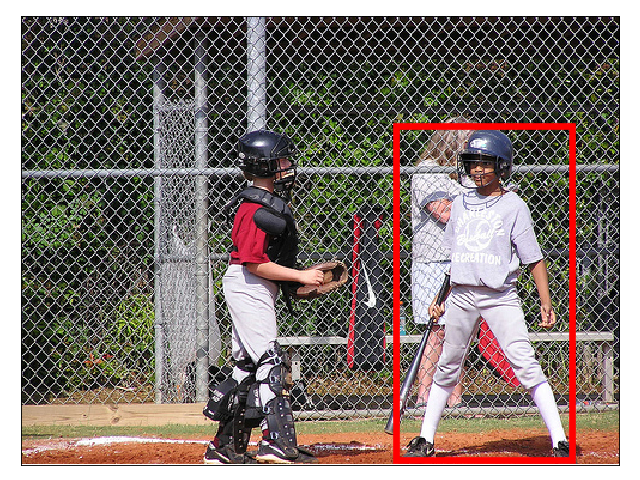
\includegraphics[width=0.9\linewidth]{figures/2398907_2901496_singleton_obj.png}}  boy (7), helmet (5), baseball player (4), player (4), man (3), child (3), batter (3), dress (2), kid (2)&
\raisebox{-\totalheight}{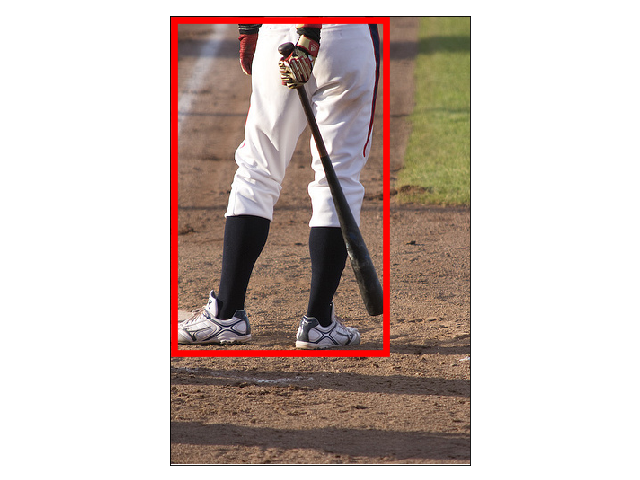
\includegraphics[width=0.9\linewidth]{figures/2337552_957263_singleton_obj.png}} pants (6), player (5), shoe (4), bat (4), person (4), legs (4), baseball player (3), hitter (2)\\ 
\multicolumn{4}{c}{\textbf{VG: robe}}\\
\raisebox{-\totalheight}{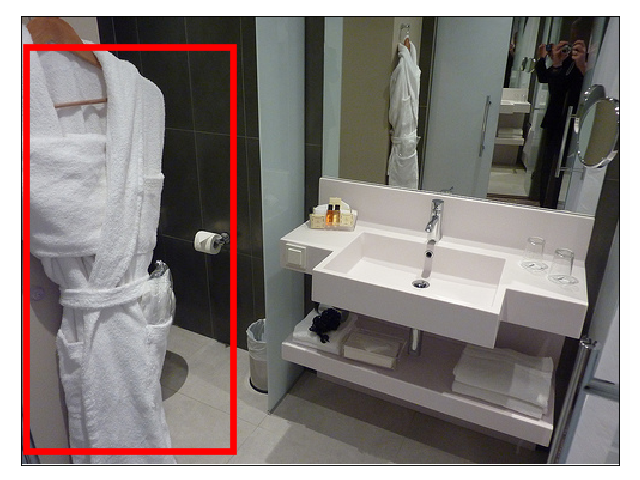
\includegraphics[width=0.9\linewidth]{figures/2373180_2333161_singleton_obj.png}} robe (27), bathrobe (5) &
  \raisebox{-\totalheight}{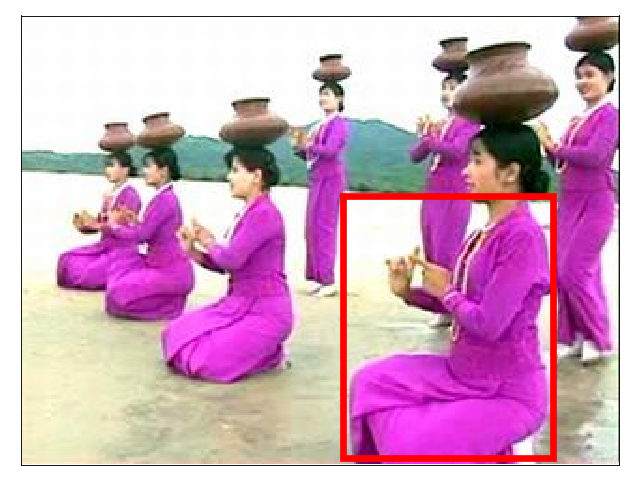
\includegraphics[width=0.9\linewidth]{figures/160_1058761_supercat_unique.png}} dress (30), uniform (2) &
\raisebox{-\totalheight}{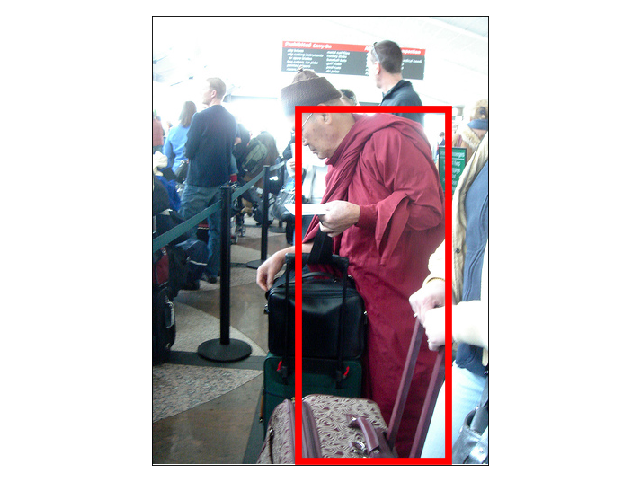
\includegraphics[width=0.9\linewidth]{figures/2334612_2838713_supercat_unique.png}}  robe (11), jacket (7), clothes (6), bag (3), dress (2), man (2) &
\raisebox{-\totalheight}{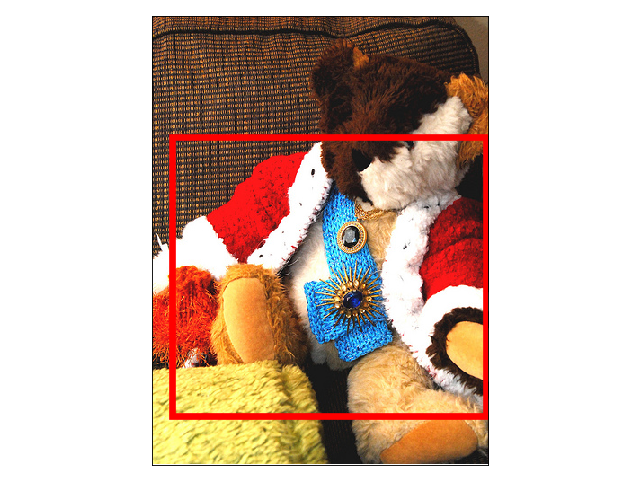
\includegraphics[width=0.9\linewidth]{figures/2340041_2137546_supercat_ambiguous.png}} jacket (10), sweater (9), coat (3), doll (3), toy (3), shirt (2), bear (2), robe (2)\\ 


\end{tabular}

}
\end{minipage}

 \caption{\label{fig:ex}Examples for different instances of VG synsets with low and high agreement in MN data set}
\end{figure*}



%\gbt{The non-canon. VG names suggest that people prefer more general names (``car $>$ sedan'', ``horse $>$ pony'', ``tie $>$ necktie''). Could be due to lexical availability (more general \ra more frequent \ra more available). This could be verified (using frequency). Hypothesis: In cases where top name != VG, the VG name is less general. Could be also a more general hypothesis: see if people prefer more frequent names in general.}
%\cs{@Table~\ref{tab:qual} (just wrt presentation) The most interesting blocks are 2 and 3 (canonical VG with min agr.; non-canonical with max agr.)}


\subsection{Discussion (for now)}
What does this discrepancy between the instance-level and category-level agreement in VisualGenome and ManyNames naming choices mean? 
First of all, it suggests that the same original VisualGenome name can trigger very different variants depending on the visual instance, leading to a drastic increase of variants elicited for categories as compared to instances.
Second, this clearly shows that annotators in VG do not generally annotate the most canonical name \cs{but they don't annotate the name, but the description} and that many names annotated for objects in VG do not correspond to the overall most preferred variant. \sz{think more ...}
\gbt{I don't think we can conclude this second part -- we do have the 70\% top=VG figure that says that VG annotators annotate the most canonical name. What this suggests to me is that instance-level properties are more important than category-level properties, somehow.
  That is, there are systematic properties of instances that make them have a single most salient name.
  However, I expect that this result will be very influenced by referential uncertainty (in single images, it will mostly be clear that it's a man, but in some it may be unclear \ra high instance agreement, low category agrement.}
\cs{I don't think that 70\% is high. E.g., the ResNet has a top-1 error rate of 25\% on ILSVRC 2015.}

\cs{(?!?) With respect to implications for L+V  models on language *interpretation*: much lower agreement on object class-level than on instance-level speaks for using very fine-grained object annotations (as done in ILSVRC). 
	However, that naming variants are often not explained/recoverable by hierarchical relations questions in how far models can understand/interpret reference to objects using more general classes (i.e., names), despite being able to recognise an object's very specific class (e.g., ILSVRC synset). (Relevant?!?)}

\begin{table*}
\footnotesize
%\begin{tabular}{p{1.3cm}cccccc|cccccc}
%\toprule
% & \multicolumn{6}{c|}{Instance-level agreement} & \multicolumn{6}{c}{Class-level agreement}\\ 
%           domain & \% top &    $H$ &    N & N$_{>1}$ & top=VG &  \% VG & \% top &    $H$ &     N & N$_{>1}$ & top=VG &  \% VG \\
%\midrule
%            all &  69.7 (22.2) &  1.3 &  5.7 &   2.9 &  72.8  &  58.7  &   52.6 (21.1) &  2.4 &   62.2 &  29.7 &  32.7 (46.9) &  23.5 (27.0)  \\
% \midrule
%         people &  51.9 (18.1) &  2.1 &  8.6 &   4.3 &         49.8 &         32.3 &     43.1 (14.9) &  2.9 &  104.4 &  53.4 &         24.4 &         13.2  \\
% animals\_plants &  91.3 (12.9) &  0.4 &  2.7 &   1.5 &         93.8 &         88.0 &     67.9 (23.5) &  1.5 &   26.7 &  12.4 &         29.5 &         26.2  \\
%       clothing &  63.9 (17.9) &  1.6 &  6.4 &   3.2 &         70.2 &         52.6 &     49.3 (16.6) &  2.6 &   71.7 &  34.1 &         40.5 &         26.1  \\
%       vehicles &  72.0 (19.5) &  1.1 &  4.7 &   2.4 &         71.1 &         60.2 &    54.4 (17.4) &  2.1 &   70.4 &  33.2 &         21.4 &         21.3  \\
%      buildings &  66.9 (20.5) &  1.5 &  6.9 &   3.0 &         72.6 &         55.5 &      46.7 (18.2) &  3.0 &   68.5 &  31.3 &         32.3 &         22.3  \\
%           home &  66.4 (20.5) &  1.5 &  6.3 &   3.1 &         78.5 &         58.8 &     49.6 (18.7) &  2.8 &  103.2 &  48.8 &         45.9 &         30.1  \\
%           food &  71.3 (21.1) &  1.3 &  5.5 &   2.9 &         62.9 &         52.1 &     47.3 (19.5) &  2.5 &   32.1 &  15.2 &         31.1 &         20.8  \\
%\bottomrule
%\end{tabular}

\begin{tabular}{lccccc|ccccc}
\toprule
 & \multicolumn{5}{c|}{Instance-level agreement} & \multicolumn{5}{c}{Class-level agreement}\\ 
          domain &    N &         \%top (std) &          H (std) & top=VG &   \%VG &     N &         \%top (std) &          H (std) & top=VG &   \%VG \\
\midrule
            all &  2.9 &  75.2 (21.9) &  0.9 (0.7) &   72.8 &  62.8 &  29.7 &  56.4 (21.5) &  2.0 (1.0) &   32.7 &  23.4 \\
       vehicles &  2.4 &  76.6 (19.8) &  0.8 (0.6) &   71.1 &  63.9 &  33.2 &  57.4 (17.3) &  1.8 (0.6) &   21.4 &  21.2 \\
      buildings &  3.0 &  74.7 (20.7) &  1.0 (0.7) &   72.6 &  61.6 &  31.3 &  51.0 (18.8) &  2.4 (0.9) &   32.3 &  22.2 \\
       clothing &  3.2 &  70.1 (18.5) &  1.1 (0.6) &   70.2 &  57.4 &  34.1 &  53.4 (16.6) &  2.1 (0.8) &   40.5 &  26.1 \\
           home &  3.1 &  72.6 (20.7) &  1.0 (0.7) &   78.5 &  64.1 &  48.8 &  54.0 (19.4) &  2.3 (1.0) &   45.9 &  29.9 \\
         people &  4.3 &  59.0 (20.4) &  1.5 (0.7) &   49.8 &  36.3 &  53.4 &  47.5 (17.2) &  2.5 (0.9) &   24.4 &  13.0 \\
           food &  2.9 &  76.4 (20.7) &  0.9 (0.7) &   62.9 &  55.2 &  15.2 &  50.8 (20.3) &  2.0 (0.8) &   31.1 &  20.8 \\
 animals\_plants &  1.5 &  94.5 (12.1) &  0.2 (0.4) &   93.8 &  91.0 &  12.4 &  71.3 (23.3) &  1.2 (0.9) &   29.5 &  26.1 \\
\bottomrule
\end{tabular}

\caption{Agreement in naming measured on the level of instances and on the level of VG classes (i.e.\ after grouping objects by their VG synset), for filtered response sets (frequency threshold of 2)}
\label{tab:agree}
\end{table*}


%Why is naming more flexible in certain domains than in others? \gbt{Hypothesis: expectation: little variation - hypernymy at most, more variation <-> more affordances <-> more varied relationships.}



\cs{@Table~\ref{tab:agree} I still think that we could also have \%\ top with $N>1$ to give an idea as to how useful the data is for the people interested in using it for, e.g., model evaluation. For that, it is clear that crowdsourcing is noisy and before using it some outlier removal needs to be made.}

% \subsection{Entry-level names and preference orders....}

% \sz{an interesting example:} In our data set, there are 24 images where \textit{penguin} has been used, so we know that the object is a \textit{penguin}. For 50\% of these images, annotators still prefer \textit{bird} as the most common name. According to the theory of entry-level categories, this should not happen. People should always prefer \textit{penguin} over \textit{bird}. 

% \sz{how can we analyze this quantitatively?}

% \begin{itemize}
% \item lettuce -- salad
% \item fruit -- food
% \item man -- catcher
% \item bowl --chili
% \item bowl -- diner \gbt{spelling mistake? should be dinner?} 
% \item burger -- meat
% \item statue -- animal (image shows statue of an animal)
% \item bottle -- alcohol
% \item donut --desert \gbt{spelling mistake? should be dessert?} 
% \item zebra -- stripes
% \item oven -- grill
% \end{itemize}


%%% Local Variables:
%%% mode: latex
%%% TeX-master: "main"
%%% End:



\section{Conclusion}

Your submission of a finalised contribution for inclusion in the LREC
proceedings automatically assigns the above-mentioned copyright to ELRA.


\section{Acknowledgements}

Place all acknowledgements (including those concerning research grants and
funding) in a separate section at the end of the article.

\section{Bibliographical References}
\label{main:ref}

\bibliographystyle{lrec}
\bibliography{naming}


%\section{Language Resource References}
%\label{lr:ref}
%\bibliographystylelanguageresource{lrec}
%\bibliographylanguageresource{lrec2020W-xample}

\end{document}
